\chapter{Praxisteil}\label{chapter:praxisteil}

Im Folgenden werden die erlangten theoretischen Erkenntnisse praktisch angewendet und so validiert.

\section{Problemstellung der betrieblichen Praxis}\label{section:problemstellung-der-betrieblichen-praxis}

Im Rahmen dieser Arbeit soll für einen Kunden der Aruba Networks eine Middleware Anwendung realisiert werden. Diese Middleware soll der Inventarisierung von Teilen der Netzwerkumgebung des Kunden dienen. 

\subsection{Die Aruba Cloud Central API}\label{subsection:die-aruba-cloud-central-api}

Der Kunde verwendet in seiner Netzwerkumgebung WLAN APs der Aruba Networks. Diese APs stellen über das Internet eine Verbindung zu der zentralen Verwaltungs- und Orchestrationseinheit Aruba Central her. Aruba Central ist ein Softwareprodukt der Aruba Networks und bietet die Möglichkeit, eine große Anzahl an APs und anderer Netzwerkgeräte in einem einzigen visuellen Benutzerinterface zu verwalten. Dabei können die Geräte weltweit an verschiedenen Standorten verteilt sein\footcite[S. 1]{hewlett_packard_enterprise_development_lp_aruba_2021-2}. Aruba Central kann sowohl vor Ort (on-premise) installiert werden, als auch aus zentralen Rechenzentren bereitgestellt werden\footcite[S. 6]{hewlett_packard_enterprise_development_lp_aruba_2021-2}. Wichtige Features der Software sind u. a. die Möglichkeit, entferntes Netzwerkequipment über das Internet  zu provisionieren, mit künstlicher Intelligenz Fehler zu finden und das Netzwerk aktiv zu überwachen\footcite[S. 1]{hewlett_packard_enterprise_development_lp_aruba_2021-2}. Vor allem das Überwachen, sprich Monitoring, ist in dieser Arbeit von Relevanz. Viele der Funktionen von Aruba Central lassen sich auch mittels einer Programmierschnittstelle bedienen\footcite[S. 6]{hewlett_packard_enterprise_development_lp_aruba_2021-2}. Für die Entwicklung der Middleware soll diese Schnittstelle verwendet werden. Die Schnittstelle wird als REST Schnittstelle bereitgestellt\footcite[S. 6]{hewlett_packard_enterprise_development_lp_aruba_2021-2}.

\subsection{Integration der Middleware in den Ivanti Endpoint Manager}\label{chapter:integration-der-middleware-in-den-ivanti-endpoint-manager}

Ein Kunde möchte die Inventardaten der APs in die Inventarisierungssoftware Ivanti Endpoint Manager importieren. Der Ivanti Endpoint Manager dient dem Inventarisieren, Verwalten, Schützen und Warten von IT Geräten\footcite[S. 3]{ivanti_inc_transparenz_2021}. 

Mit dem Kunden wurde die Vereinbarung getroffen, dass lediglich ein Prototyp der Middleware für die JavaScript Laufzeitumgebung V8 entwickelt wird und der Kunde diesen Prototyp selbst in die Software integriert. Die Software Ivanti Endpoint Manager findet aus diesem Grund keine weitere Betrachtung.

\subsection{Anforderungen an die Middleware}\label{subsection:anforderungen-an-die-middleware}

Das praktische Ziel dieser Arbeit ist ein Middleware Skript zu entwickeln, welches sich mit der REST API von Aruba Cloud Central verbindet und Inventardaten über die Aruba Access Points abfragt. Die Daten soll das Skript dann in einer verkürzten Form ausgeben.

Im Folgenden werden nach ISO 25010\footcite{isoiec_25010_isoiec_2011} sowohl funktionale als auch nicht-funktionale Anforderungen an das Programm aufgestellt. Aufgrund einer langjährigen Vertrauensbasis mit dem Kunden konnten die Anforderungen informell festgelegt werden. So besteht keinerlei schriftliche Dokumentation der Anforderungen. Im Folgenden werden diese stichwortartig aufgelistet:

\textbf{Funktionale Anforderungen}

\begin{enumerate}
    \item Das Skript soll sich mittels Kundendaten mit der Aruba Cloud Central API authentifizieren.
    \item Daten über alle Access Points der Netzwerkumgebung sollen gesammelt werden. Diese Daten werden zunächst im Arbeitsspeicher zwischengespeichert.
    \item Ein Auszug der Daten soll auf dem Bildschirm ausgegeben werden. 
\end{enumerate}

\textbf{Nicht-Funktionale Anforderungen}

\begin{enumerate}
    \item Die Anwendung muss mit der Programmiersprache JavaScript umgesetzt werden und auf der JavaScript Runtime V8 ausführbar sein.
    \item Sie soll umfangreich kommentiert, dokumentiert und so wenig komplex wie möglich sein.
    \item Die Anwendung soll Plattformunabhängig sein.
    
\end{enumerate}

\section{Analyse des Access Point Monitoring API Endpunktes}\label{section:analyse-des-access-point-monitoring-endpunkte}

Für das Umsetzen der Middleware muss ein API Endpunkt angesprochen werden. In mehreren Studien wurde jedoch festgestellt, dass in der Praxis viele APIs nicht komplett dem REST Architekturstil entsprechen \footnote{Vgl. \cite[S. 243]{franch_detection_2014}, \cite[S. 185]{palma_semantic_2017}, \cite[S. 11f]{presutti_restful_2014} und \cite[S. 38]{rodriguez_restful_2008}}. Dies könnte also auch bei der Aruba Central API der Fall sein. Da es für die Umsetzung der Middleware unabdinglich ist, dass die Aruba API REST konform ist, wird im Folgenden analysiert, ob die API den REST Regeln entspricht. Hierbei wird auf die in Kapitel \ref{section:klassifizierung-von-rest} definierten Regeln im Gütemodell von Richardson zurückgegriffen.

Zunächst ist es erforderlich, sich mit der API zu authentifizieren. Die Authentifizierung folgt dem OAuth2 Standard\cite{parecki_oauth_2021} und erfordert drei Abfragen. Der genaue Ablauf der Authentifizierungsroutine ist auf einer öffentlichen Dokumentationsseite der Aruba Networks dokumentiert\cite{hewlett_packard_enterprise_development_lp_oauth_2021} und wird hier nicht weiter betrachtet.

Nach der erfolgreichen Authentifizierung können Daten von der API abgerufen werden. Die Statusdaten der APs werden mit einem Endpunkt bzw. einer Ressource der API angeboten\footcite{hewlett_packard_enterprise_development_lp_aruba_2021-1}. Im Folgenden wird dieser Endpunkt genauer untersucht. Sowohl das Abrufen der Daten vom Endpunkt, als auch der Rückgabewert werden beschrieben und argumentativ deduktiv analysiert. 

Für die Beschreibung des API Endpunktes wurden mit dem HTTP-Client Postman\footcite{postman_inc_postman_2021} HTTP-Abfragen an die API gesendet. Das Resultat dieser Abfragen wurde gespeichert und dem Anhang dieser Projektarbeit beigefügt. Im Folgenden werden lediglich Ausschnitte der Abfrage betrachtet. Die Zeilennummern am linken Rand der Abfrage im Text verweisen dabei auf die Zeilennummern aus der ursprünglichen kompletten Abfrage im Anhang.

\subsection{Abfrage des Monitoring Endpoints}\label{subsection:abfrage-des-monitoring-endpunktes}

Zunächst wird die Abfrage der Statusinformationen von der API betrachtet. Im Folgenden werden Auszüge der Abfrage als unveränderter Text gezeigt.

\begin{lstlisting}
GET /monitoring/v2/aps HTTP/1.1
Host: internal-apigw.central.arubanetworks.com  
\end{lstlisting}

Die einzelnen Bestandteile der Abfrage werden im Folgenden analysiert.

\emph{Protokollversion (Zeile 1)}: Am Ende von Zeile 1 wird angegeben, dass die Abfrage der Version 1.1 des HTTP-Protokolls entspricht. Diese Version des HTTP-Protokolls wird in RFC 2616 beschrieben. Stimmt der Rest der Abfrage ebenfalls mit HTTP/1.1 überein, ist Level 0 des Gütemodells von Richardson erfüllt.

\emph{Analyse der URL (Zeile 1 und 7)}: Aus Zeile 1 und Zeile 7 lässt sich die Uniform Ressource Locator (URL) der Ressource erkennen. Zusammengesetzt ist sie hier zu sehen:

\emph{https://internal-apigw.central.arubanetworks.com/monitoring/v2/aps}

Nun wird untersucht, ob der Aruba Monitoring Endpunkt dem generellen Aufbau einer URL folgt. Hierzu wird versucht, die einzelnen Bestandteile der URL den generischen Bestandteilen von URLs zuzuweisen. Abbildung \ref{abb:AufbauArubaURL} illustriert diese Zuordnung

\begin{figure}[htb]
\centering
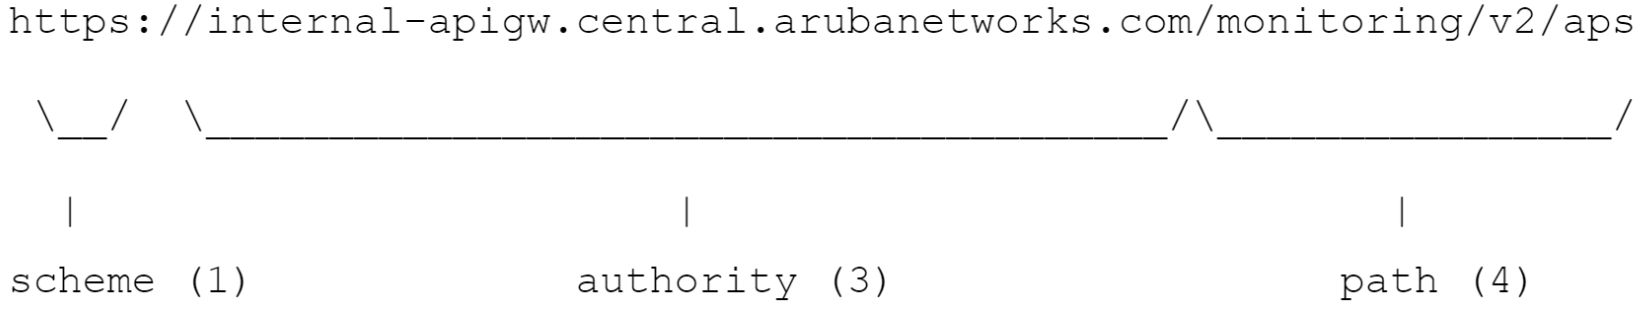
\includegraphics[width=12cm]{graphics/aufbau-aruba-url.png}
\caption[aufbau-aruba-url]{Aufbau der URL des Aruba Endpunktes.}
\label{abb:AufbauArubaURL}
\end{figure}

In der Abbildung ist erkennbar, dass alle obligatorischen Elemente (1-4) syntaktisch korrekt vorhanden sind. Somit entspricht die URL des Endpunktes dem RFC 3986.

Der Aufbau der URL lässt auch auf die Struktur der API schließen. Alle Autoren der zuvor genannten Quellen sind sich einig, dass es möglich sein muss, Ressourcen eindeutig über URLs zu identifizieren\footcite{fowler_richardson_2010}. In der URL folgen die Begriffe monitoring, v2 und aps aufeinander. Nach Tilkov ergibt sich aus der URL eine natürliche, hierarchische Anordnung\footcite[S. 40]{tilkov_rest_2015}. Nach Hesse stellt monitoring eine Collection, sprich eine Sammlung von Elementen dar. Der Pfad-Bestandteil v2 ist ebenfalls eine Collection und ist ein Teil von monitoring. Zuletzt ist aps eine Ressource in der v2 collection. Aus der obigen URL ist somit eine klare Struktur der API erkennbar\footcite[S. 12]{masse_rest_2012}. 

Analyse des HTTP Verbes (Zeile 1): In Zeile 1 ist zu erkennen, dass der Request Methoden Token\footcite[S. 36]{fielding_hypertext_1999} GET ist\footcite[S. 53]{fielding_hypertext_1999}. 

\begin{lstlisting}
GET /monitoring/v2/aps HTTP/1.1
\end{lstlisting}

Der Zweck des Endpunktes ist es, Informationen zu den APs im Netzwerk abzurufen\footcite{hewlett_packard_enterprise_development_lp_aruba_2021-1}. Es werden keine Informationen auf dem Server verändert und keine Aktionen ausgelöst. Laut RFC 2616 (Das HTTP Protokoll) ist genau für eine solche Operation die GET Methode sinnvoll\footcite[S. 53]{fielding_hypertext_1999}. Durch adäquate Request Methoden kann der Zweck einer Operation geschlussfolgert werden. Zum Beispiel kann so gesagt werden, dass der vorliegende Endpunkt idempotent ist und theoretisch gecacht werden dürfte\footcite[S. 24 und 26]{masse_rest_2012}. Auch Hesse unterstützt die Aussage, dass GET in diesem Fall die richtige Request Methode ist.

Zusammengefasst konnten in der HTTP Abfrage eine korrekte Request Methode, eine korrekte URL, sowie HTTP/1.1 als Protokollversion festgestellt werden. Durch das Verwenden von HTTP besteht die Abfrage Level 0 des Gütemodells. Durch die korrekte URL wird Level 1 bestanden und durch den korrekten Pfad Level 2.

\subsection{Antwort des Monitoring Endpoints}\label{subsection:antwort-des-monitoring-endpunktes}

Auf die HTTP-Abfrage des Endpunktes sollte der Monitoring Endpunkt die Inventardaten der WLAN-APs zurückgeben. Der Rückgabewert der Abfrage ist im folgenden Code zu sehen.

\small
\lstset{firstnumber=1}
\begin{lstlisting}
HTTP/1.1 200 OK
Content-Type: application/json
Transfer-Encoding: chunked
Date: Sat, 31 Jul 2021 11:36:35 GMT
cache-control: no-cache, no-store, must-revalidate, private
Content-Encoding: gzip
 
{
	"aps": [
		{
			"ap_deployment_mode": "IAP",
			"ap_group": null,
			"cluster_id": "",
			"controller_name": "",
			"group_name": "dw_AP-Group",
			"ip_address": "192.168.0.14",
			"labels": [],
			"last_modified": 1627371453,
			"name": "ctrl-dw01",
			"public_ip_address": "95.91.239.249",
			"status": "Up",
		},
...    
\end{lstlisting}

\emph{Der Status Code (Zeile 12):}
Die erste Zeile der HTTP Antwort kann dem folgenden Code entnommen werden.

\lstset{firstnumber=12}
\begin{lstlisting}
HTTP/1.1 200 OK
\end{lstlisting}

Laut dem HTTP Protokoll sollte die erste Zeile einer HTTP Antwort aus der Protokollversion, einem dreistelligen Status Code und einer kurzen textuellen Beschreibung des Status Codes bestehen\footcite[S. 39]{fielding_hypertext_1999}. In der vorliegenden Antwort wurde der Status Code 200 zurückgegeben. Dieser besagt, dass die angefragten Informationen erfolgreich abgerufen werden konnten\footcite[S. 58]{fielding_hypertext_1999}. Wie in den folgenden Textpassagen erkenntlich wird, konnten die Informationen tatsächlich erfolgreich zurückgegeben werden. Der Statuscode ist somit an dieser Stelle angebracht.

\emph{Content Type und Encoding (Zeile 13, 14 und 27):} 

In der Zeile 13, 14 und 16 der Antwort werden genauere Informationen über die Formatierung des Inhalts der Antwort übergeben (Code folgend). 

\lstset{firstnumber=13}
\begin{lstlisting}
Content-Type: application/json
Transfer-Encoding: chunked
Content-Encoding: gzip
\end{lstlisting}

Nach dem HTTP Protokoll gehören die Header Content-Type (Zeile 13) und Content-Encoding zu den Entitäts Kopfdaten\footcite[S. 42]{fielding_hypertext_1999}. Diese Kopfdaten sollen zusätzliche Metainformationen über den Inhalt der Antwort geben. In Fieldings Vokabular beschrieben, bezeichnen sie den Typ der Repräsentation einer Ressource\footcite[S. 88ff]{fielding_architectural_2000}. Der Content-Type Header spezifiziert den genauen Typ des Inhalts. Hier wird ein JavaScript Object Notation (JSON) Dokument erwartet\footcite[S. 1]{crockford_applicationjson_2006}. Weitere Typen wurden in weiteren RFCs definiert. Der Content-Encoding Header spezifiziert eine zusätzliche Encodierung des Inhalts\footcite[S. 168]{berners-lee_univeral_1996}. In diesem Beispiel wird das JSON Dokument zusätzlich mit der GZIP Komprimierung encodiert. Mit dem Transfer-Encoding Header wird festgelegt, ob Veränderungen an dem Inhalt der Nachricht vorgenommen wurden, um sie zu transportieren\footcite[S. 143]{berners-lee_univeral_1996}. So kann, wie in diesem Beispiel, der Inhalt aufgeteilt werden, um ihn schneller und sicherer zu transportieren\footcite[S. 143]{berners-lee_univeral_1996}.

\emph{Date und Cache Control (Zeile 18 und 21)}

In den Zeilen 18 und 21 werden der Date und der cache-control Header gesetzt (im folgenden Code zu sehen).

\lstset{firstnumber=18}
\begin{lstlisting}
Date: Sat, 31 Jul 2021 11:36:35 GMT
\end{lstlisting}

\lstset{firstnumber=21}
\begin{lstlisting}
cache-control: no-cache, no-store, must-revalidate, private
\end{lstlisting}

Bis auf wenige Ausnahmefälle (beschrieben in Kapitel 14.18 des RFC 2616\footcite[S. 124]{berners-lee_univeral_1996}) muss jede Antwort eines Servers den genauen Absendezeitpunkt beinhalten. Die Zeitangabe muss dabei nach RFC 1123 formatiert sein\footcite[S. 124]{berners-lee_univeral_1996}. Sie kann später von Server und Client zu Entscheidungen bezüglich des Cachings der Ressource genutzt werden.

Der Header cache-control beschreibt, ob und wie eine Antwort zwischengespeichert werden soll. Der Header kann sowohl vom Client, als auch vom Server gesetzt werden. Bei einem Konflikt soll die restriktivste Caching Methode verwendet werden\footcite[S. 77]{berners-lee_univeral_1996}. In der vorliegenden Antwort des Servers werden die cache-control directives no-cache, no-store, must-revalidate und private gesetzt. Diese besagen, dass die Ergebnisse der Abfrage nicht wiederverwendet (no-cache\footcite[S. 109]{berners-lee_univeral_1996}) und nicht zwischengespeichert (no-store\footcite[S. 110]{berners-lee_univeral_1996}) werden dürfen. Sie müssen stetig neu validiert werden (must-revalidate\footcite[S. 113]{berners-lee_univeral_1996}) und dürfen nicht in einem geteilten Cache abgelegt werden (private\footcite[S. 109f]{berners-lee_univeral_1996}). Die Informationen sind hochsensibel, also scheint eine solche Caching Richtlinie sinnvoll. Durch die zuvor genannten Cache Header wird genau angegeben, ob die Ressource cachebar ist oder nicht. Somit wird die dritte Randbedingung Fieldings erfüllt. Auch Richardson empfiehlt klar, dass ein Server angeben sollte, dass eine Ressource nicht cachebar ist\footcite[S. 248]{richardson_restful_2007}.

\emph{Der Body der Antwort (Ab Zeile 32)}

Wie zuvor beschrieben, sieht der Status Code 200 einer Antwort vor, dass die Antwort einen Inhalt enthält. Wie zuvor erläutert, sollte es nach dem HATEOS Prinzip möglich sein, allein mittels Hyperlinks durch eine API zu navigieren. In dem vorliegenden Auszug des Nachrichteninhalts sind mehrere Bezüge zu anderen Entitäten klar erkennbar: So könnten ap\_group (Zeile 36) und controller\_name (Zeile 38) auf andere Ressourcen verweisen. Anstatt von Hyperlinks finden sich hier jedoch die Namen der jeweiligen Ressourcen wieder. Ohne vorherige Kenntnis der API Struktur ist es somit nicht möglich, mehr Informationen über z.B. die Gruppe des Access Points abzurufen.

Zusammengefasst erfüllt die Antwort des Monitoring Endpunktes mit korrekten HTTP Headern Level 0 des Gütemodells. Level 1 ist hier nur für die Abfrage relevant. Level 2 wird erfüllt dar ein korrekter Response Status Code zurückgegeben wird. Level 3 wird nicht erfüllt, da in der Antwort keine Hypermedia Referenzen verwendet werden.

\subsection{Einordnung in das Richardson Reifegradmodell}\label{subsection:einordnung-in-das-richardson-reifegradmodell}

Nachdem der Monitoring Endpunkt zuvor analysiert wurde, wird er nun in das Reifegradmodell von Richardson eingeordnet. Level 0 (HTTP) ist bestanden, da sowohl Abfrage, als auch Antwort nach HTTP/1.1 korrekte beschrieben sind. Level 1 (Ressourcen) wird durch die korrekte URL in der Abfrage erfüllt. Level 2 durch korrekte HTTP Verben und Status Codes. Level 3 wird nicht erfüllt, da das HATEOS Prinzip nicht beachtet wird. Aufgrund dieser Beobachtungen ist anzunehmen, dass eine Implementierung der Middleware eingeschränkt möglich ist (Level 0 bis 2). Es müssen jedoch Informationen zur Struktur der API in den Client eingebaut werden, dar diese nicht durch Hypermedia Referenzen automatisiert abrufbar sind. Das Forschungsergebnis wird im folgenden Kapitel mittels Prototyping validiert.

\section{Evaluierung des Analyseergebnisses durch Prototyping}\label{section:Evaluierung-des-Analyseergebnisses-durch-Prototyping}

Mittels einer argumentativ deduktiven Analyse konnte festgestellt werden, dass die Aruba Cloud Central API überwiegend den REST Best Practices entspricht. Dieses Forschungsergebnis soll validiert werden. Best Practice Empfehlungen verfolgen i.d.R. den Zweck, die Geschwindigkeit und Qualität einer Implementierung zu erhöhen. Entspricht die Aruba Cloud Central API den Best Practices, ist folglich anzunehmen, dass eine Umsetzung der Middleware mit vergleichsweise geringen Aufwand vollzogen werden kann.

\subsection{Genereller Programmablauf}\label{subsection:genereller-programmablauf}

Das Middleware Programm besteht im Wesentlichen aus HTTP Anfragen an die Aruba Cloud Central REST API. HTTP Anfragen sind in ihrer Natur asynchron. JavaScript ermöglicht es ebenfalls, in einer asynchronen Art zu programmieren. Demnach liegt es auch auf der Hand, das Inventarisierungsprogramm asynchron zu gestalten. In JavaScript stehen eine Reihe von Mechanismen zur asynchronen Programmierung zur Verfügung. Ein sehr verbreiteter Ansatz ist der der Promises\footcite[S. 11]{parker_javascript_2015}. Dieser Ansatz wird auch in dem Skript verfolgt. Speziell werden in der Anwendung verschiedene HTTP Anfragen in einer sog. Promise Chain der Reihe nach abgearbeitet. Auch die verwendete Bibliothek Axios unterstützt das Arbeiten mit einer Promise Chain\footcite{zabriskie_axios_2021}. 

Zunächst wird der Authentifizierungsendpunkt aufgerufen (Zeile 12 bis 20). Dieser Aufruf gibt ein Promise zurück\footcite{zabriskie_axios_2021}. In einem nächsten Funktionsaufruf werden die zuvor abgerufenen Authentifizierungsinformationen abgespeichert (Zeile 21 bis 41). Das komplette Authentifizierungsverfahren wird hier nicht weiter erklärt, da sie unabhängig von dem analysierten Endpunkt geschieht. Mit den Authentifizierungsinformationen werden dann die Inventardaten der Access Points abgerufen (Zeile 42 bis 51, Kapitel \ref{subsection:abrufen-der-Inventardaten}). Zuletzt werden die gesammelten Daten ausgegeben (Zeile 52 bis 62, Kapitel \ref{subsection:ausgeben-der-Inventardaten}). In Zeile 63 bis 65 wird über die Catch Methode ein Error Handler an alle Promises gehängt\footcite[S. 772]{ecma_international_ecmascript_2021}. Sollte einer der zuvor genannten Schritte mit einer Exception abgebrochen werden, wird die Promise Chain abgebrochen und der Fehler wird mit dem catch Block behandelt\footcite{mozilla_foundation_using_2021}.

\subsection{Umgebungsvariablen}\label{subsection:Umgebungsvariablen}

Für die Authentifizierung mit der API sind Zugangsdaten erforderlich. Die Zugangsdaten werden dem Programm in sogenannten Umgebungsvariablen zur Verfügung gestellt. So ist garantiert, dass keine sensiblen Daten in dem Programmcode aufzufinden sind. Tabelle .. zeigt eine Erklärung der Umgebungsvariablen:


\begin{table}[htb]
\centering
\begin{tabular}{l|l}
    \textbf{Variable} & \textbf{Erklärung} \\
    \hline
    ARUBA\_CENTRAL\_API\_ROOT\_PATH & Der Basis Pfad der Aruba Central API \\
    \hline
    ARUBA\_CENTRAL\_CLIENT\_ID & Die Client ID als Sicherheitsmerkmal \\
    \hline
    ARUBA\_CENTRAL\_CLIENT\_SECRET & Das Client Secret als Sicherheitsmerkmal \\
\end{tabular}
\caption{Umgebungsvariablen.}
\label{tab:Umgebungsvariablen}
\end{table}

\subsection{Abrufen der Inventardaten}\label{subsection:abrufen-der-Inventardaten}

Nach der erfolgreichen Authentifizierung mit der Aruba API können die Inventardaten abgerufen werden (Zeile 42 bis 51). Alle vom Kunden geforderten Daten lassen sich mittels eines API Endpunktes abrufen. Dieser Endpunkt wurde bereits in Kapitel \ref{section:analyse-des-access-point-monitoring-endpunkte} beschrieben. 

\lstset{
    firstnumber=45,
    breaklines=true
}
\begin{lstlisting}
return axios.get(process.env.ARUBA_CENTRAL_API_ROOT_PATH + 'monitoring/v2/aps',
{
    headers: {
    Authorization: `Bearer ${tokenStore.readTokenObject().access_token}`
    }
})    
\end{lstlisting}

Die Abfrage besteht aus dem Funktionsaufruf der axios.get Funktion. Die axios.get Funktion wird in der offiziellen Dokumentation von Axios erläutert\footcite{zabriskie_axios_2021-1}. Mit ihr ist es möglich, eine GET Anfrage an eine bestimmte URL zu senden. 

Als erster Parameter wird bei der axios.get Methode die URL angegeben (Zeile 45). Diese URL entspricht der URL des zuvor in Kapitel analysierten Monitoring Endpunktes. Neben der URL ist für eine erfolgreiche Abfrage lediglich der Access Token notwendig. Dem OAuth2 Standard entsprechend wird dieser Token in einem Authorization Header mit der Abfrage an den Server geschickt. Header können mit Axios mit der headers Konfigurationsoption gesetzt werden\footcite{zabriskie_axios_2021}. In Zeile 47 bis 49 wird ein Authorization Header mit dem Access Token an die Abfrage angehängt. Mit dem Aufrufen der Funktion wird die HTTP Anfrage abgeschickt und ein Promis für die Erfüllung der Abfrage zurückgegeben. Im Promise wird danach mit der then Funktion eine Funktion hinterlegt, welche die abgerufenen AP Daten in der Konsole ausgibt.

\subsection{Ausgeben der Inventardaten}\label{subsection:ausgeben-der-Inventardaten}

Ist die Abfrage der Monitoring Informationen erfolgreich werden diese in der Programm Konsole ausgegeben. Da die vorliegende Version der Software lediglich ein Prototyp ist, genügt diese Ausgabe den Anforderungen (siehe Kapitel \ref{subsection:anforderungen-an-die-middleware}). In der fertiggestellten Middleware werden die Informationen an dieser Stelle in das Inventarisierungsprogramm des Kunden geladen. 

In diesem Beispiel werden die Access Point Daten zunächst aus der Antwort des Servers extrahiert (Zeile 55). Dann wird mit einer Schleife über die Objekte der einzelnen Access Points iteriert (Zeile 58) und jeweils beispielhaft der Name des APs ausgegeben (Zeile 59).
Sind die Daten erfolgreich ausgegeben hat die Middleware an dieser Stelle alle Anforderungen erfüllt. Trat bei einem der zuvor genannten Schritte ein Fehler auf, tritt die in Kapitel \ref{subsection:genereller-programmablauf} erklärte Fehlerbehandlung in Kraft.



